A Point-Of-Presence (POP) is an artificial demarcation point or interface point between communicating entities. Al POPs mentioned in this documents refers to optical fiber (OF) interconnection points.

Since 2010 the guifi.net community has raised five POPs over the Catalan territory, all of them according to the Bottom-up Broadband (BuB) model specified in the guifi.net network license\footnote{This is the agreement all users must accept to join the network. It's mission is to keep the network free, open and neutral. The Catalan version can be found at \url{http://guifi.net/ca/CXOLN}. It has not yet been translated into English}.
Thus anyone is able to connect to them as long as he/she accepts this license.

From a general perspective guifi.net community is building a set of neutral exchange points, leaving the infrastructure available to the individuals, associations or either companies. These kind of POPs are named POP-IX referring to the Internet eXchange points (IX).

Figure \ref{fig:fibre_map} shows the OF network map of guifi.net POPs as of December 2012. The backbone, i.e. the POPs interconnections are made using third party infrastructures. Currently all the POP interconnection links are over the Xarxa Oberta de Catalunya (XOC)\footnote{\url{http://www.xarxaoberta.cat/en/about-xoc}}.

\begin{figure}[htbp]
  \centering
  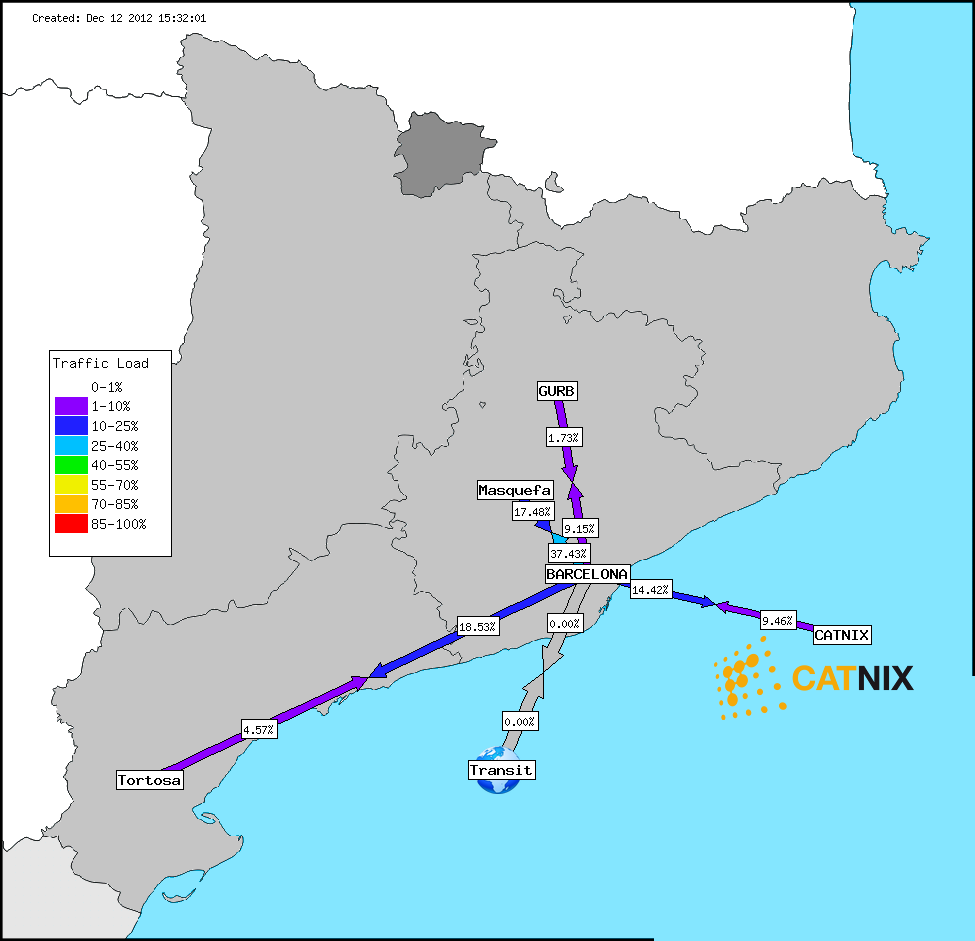
\includegraphics[scale=.35]{sect3/figures/pops_network_map.eps} 
  \caption{Guifi.net fiber POPs network map}
  \label{fig:fibre_map}
\end{figure}


\FloatBarrier
\subsection{Pilot's POPs}

\FloatBarrier
\subsubsection{Gurb}
Gurb pilot has its own POP fully operational. The POP is placed in the garage of a home's guifi.net member. The garage also hosts a data center where the guifi.net partners\footnote{A guifi.net partner is a guifi.net member that has professional interest in the network.} can collocate their hardware. Pictures on Figure~\ref{fig:gurb_net_load} shows some details of the current installation.


\begin{figure}[htbp]
  \centering
    \begin{tabular}{cc}
      \resizebox{70mm}{!}{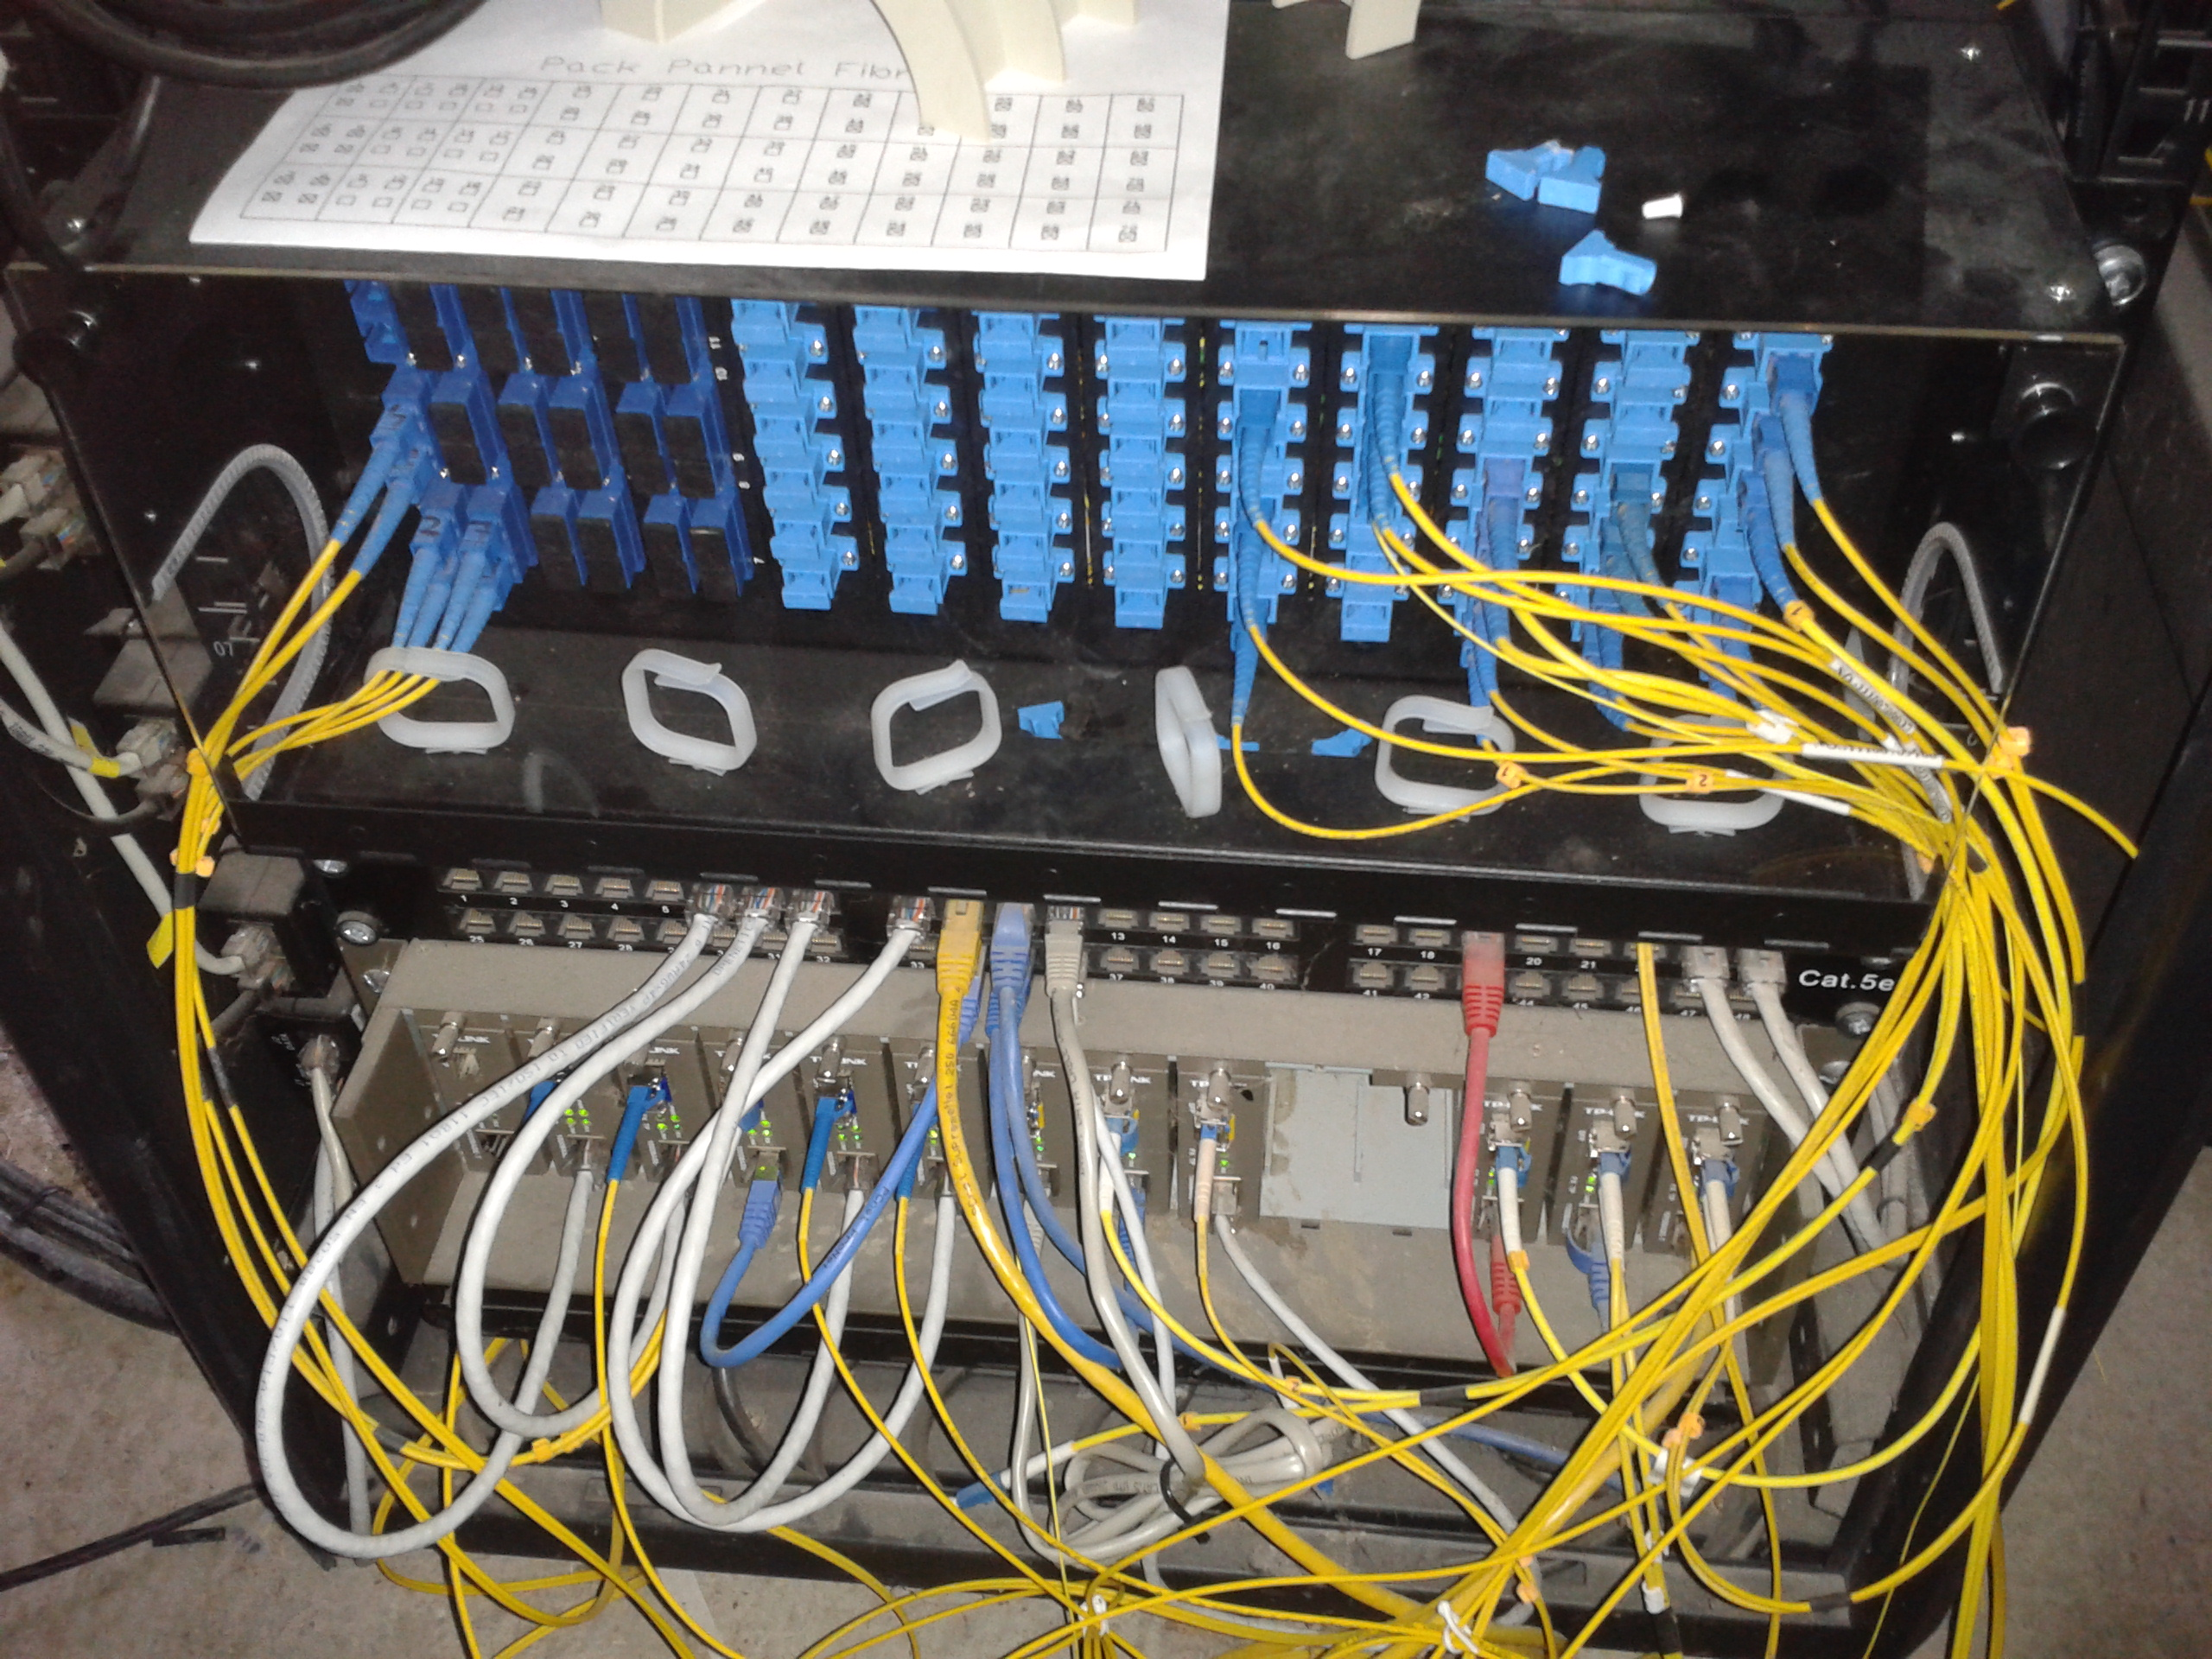
\includegraphics{sect3/figures/gurb_rack1.eps}} &
      \resizebox{70mm}{!}{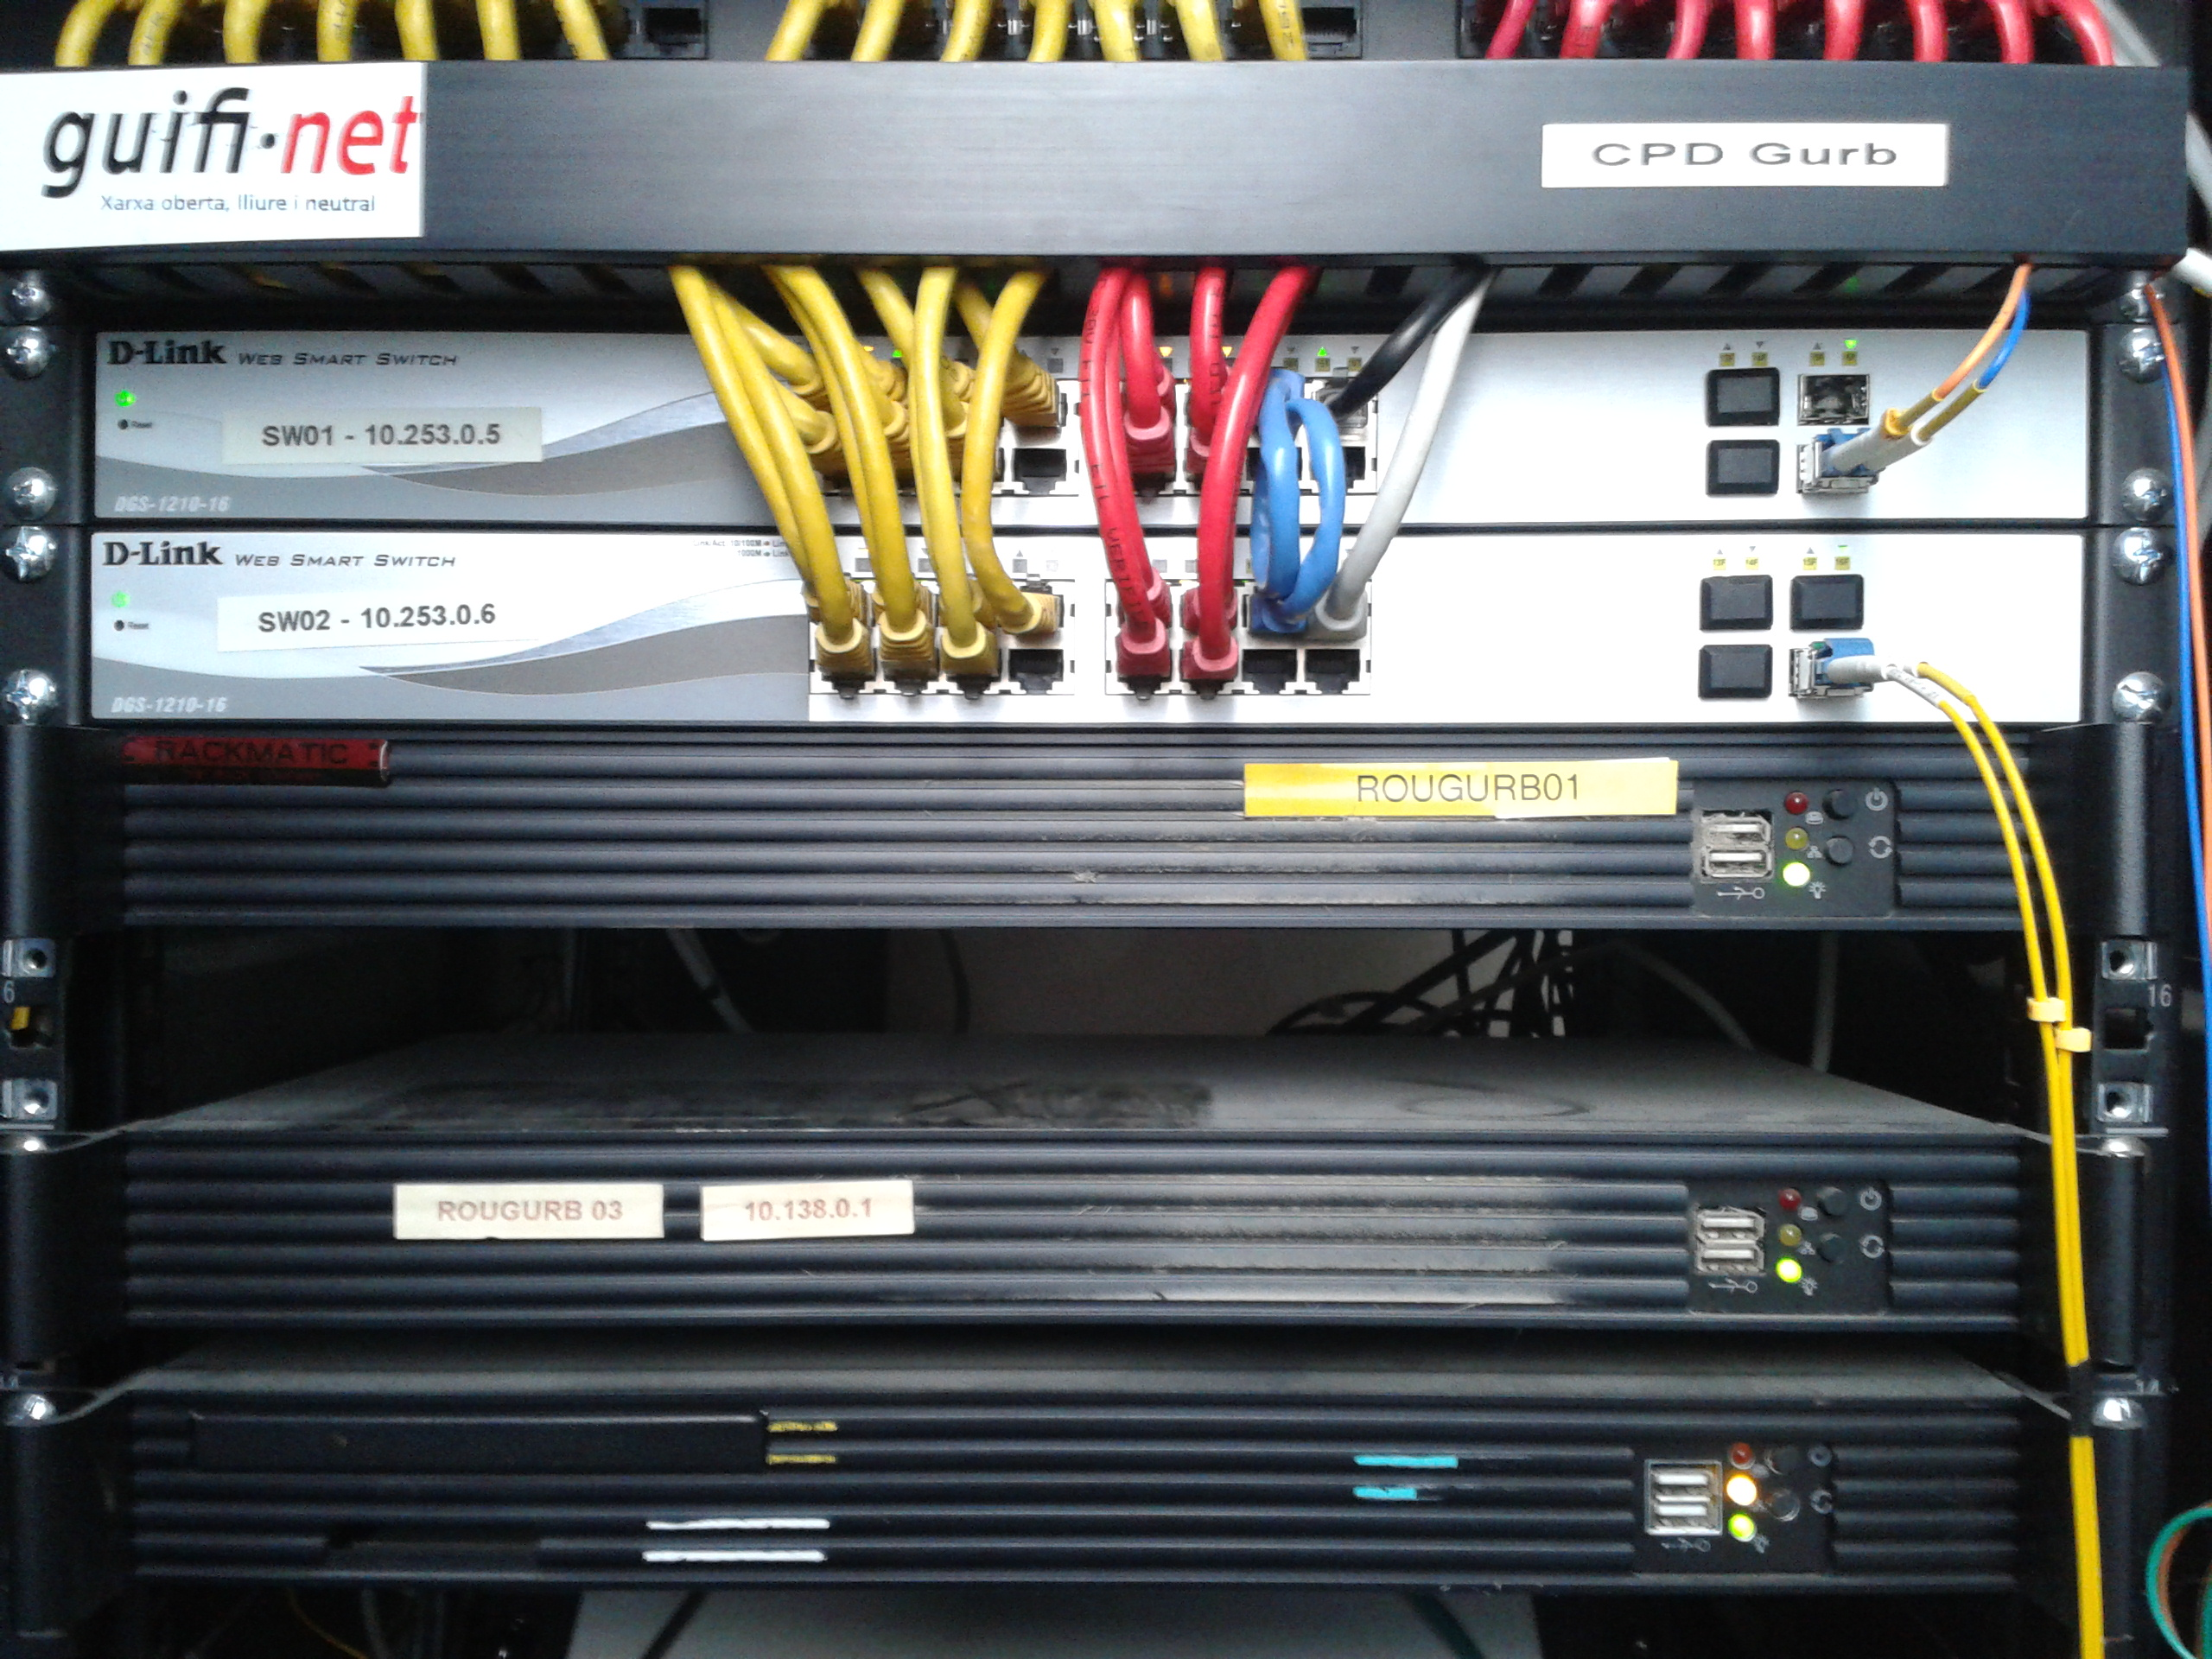
\includegraphics{sect3/figures/gurb_rack2.eps}} \\
    \end{tabular}
  \caption{Gurb's POP detailed pictures. On the right the OF terminations. On the left the routers.}
  \label{fig:grub_rack}
\end{figure}

This POP, activated in 2010, was the first one. Figure~\ref{fig:gurb_net_load} shows its traffic load in 2012.

\begin{figure}[htbp]
  \centering
  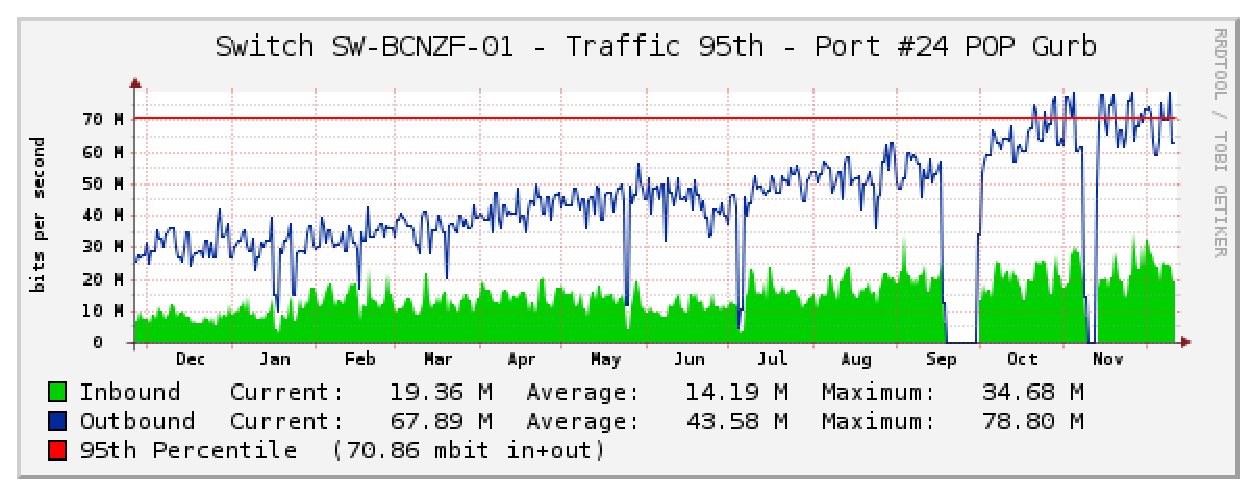
\includegraphics[scale=.65]{sect3/figures/gurb_network_load_year.eps} 
  \caption{Gurb's POP network load (year 2012).}
  \label{fig:gurb_net_load}
\end{figure}


\FloatBarrier
\subsubsection{Vic}

The Vic's POP is expected to be fully activated in the coming days.


\FloatBarrier
\subsection{Other POPs}


\FloatBarrier
\subsubsection{Telvent-Barcelona}

Telvent-Barcelona is a commercial data center\footnote{\url{http://www.telvent.es/en/}} placed in an industrial park of Barcelona. It hosts the CATNIX\footnote{\url{http://www.catnix.net}}, the Internet exchange point (IX) of Catalonia, a physical infrastructure provided by the Catalan government. IXs are critical for the Internet since they are meant to let the network operators exchange their information and connect their networks (autonomous systems). 

On the one hand, as be shown in Figure \ref{fig:fibre_map}, all guifi.net POPs are linked to TELVENT-Barcelona. On the other hand, guifi.net connects to the Internet through this POP.

guifi.net Foundation operates it's own backbone infrastructure using the ASN 49835 (Autonomous System Number). 
An open peering policy is followed to establish peering sessions with all potential partners. Figure~\ref{fig:catnix_net_load} shows the total peering traffic of guifi.net CATNIX port\footnote{To be a CATNIX members must have at least one public ASN and one public IP block. Guifi.net is a Local Internet Registry (LIR) since it is a RIPE-NCC member, and has its own ASN numbers and IPv4 and IPv6 blocks.}. Additionally guifi.net Foundation has an Internet Gigabit uplink contracted with Cogent\footnote{\url{http://www.cogentco.com/en/}}. Figure~\ref{fig:cogent_load} . All guifi.net Foundation routers and servers are allocated in a 22U rack in Telvent-Barcelona, shown in Figure~\ref{fig:telvent_rack}. 


Figure \ref{fig:telvent_scheme} shows a connection scheme (layer 2) of the hardware used for the CATNIX POP. 
The first port of the switch SW-03 is the optical fiber which brings the data from the other POPs. As can be seen each
of them use a separate VLAN. The seventh port of the second switch is the connection with the carrier to reach the Internet.
And the eight is connected to the CATNIX infrastructure where the exchange of data with other ISPs and networks is possible. 


The Telvent-Barcelona Foundation resources are shared with other partners, such as puntCat\footnote{\url{http://www.domini.cat/}}, the Catalan Top-Level Domain (TDL), which is currently using half of the space available.

\begin{figure}[htbp]
  \centering
  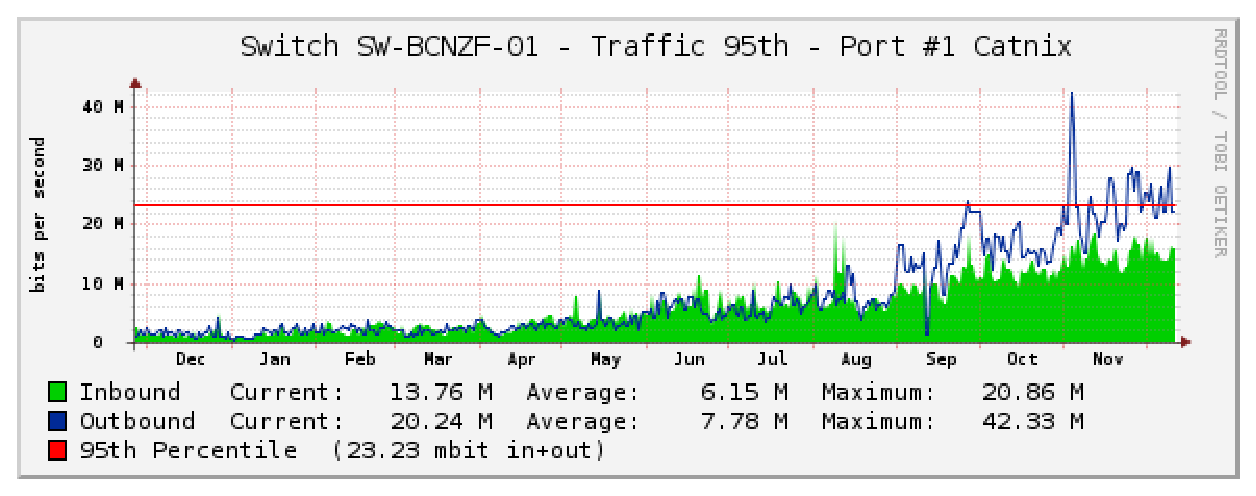
\includegraphics[scale=.65]{sect3/figures/catnix_network_load_year.eps} 
  \caption{Telvent-Barcelona's POP network load (year 2012).}
  \label{fig:catnix_net_load}
\end{figure}


\begin{figure}[htbp]
  \centering
  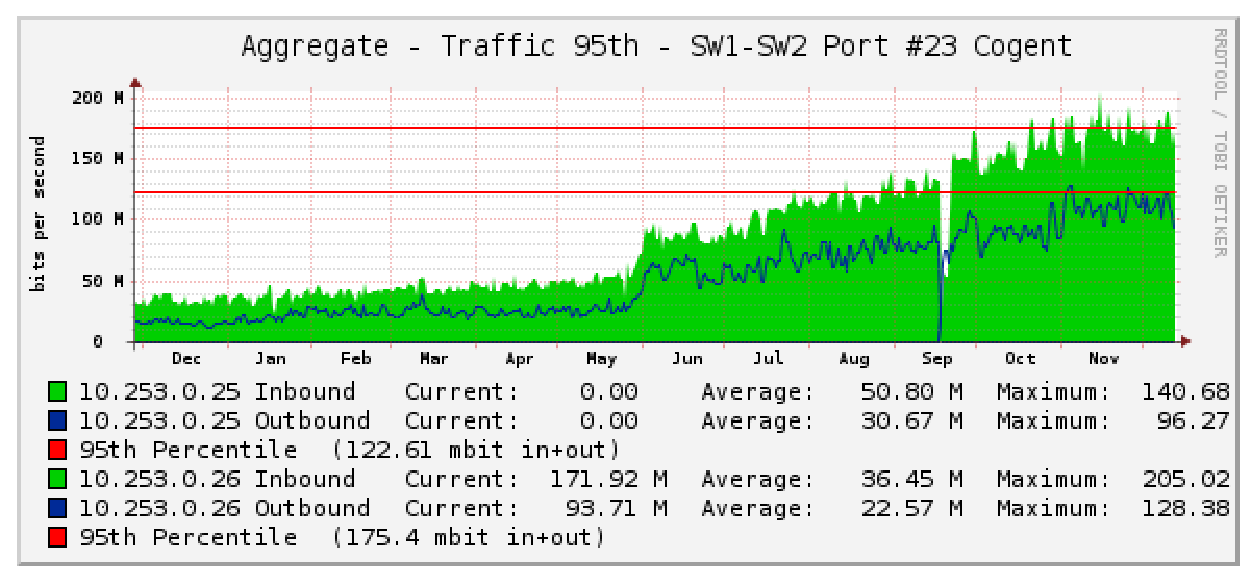
\includegraphics[scale=.65]{sect3/figures/cogent_network_load2.eps} 
  \caption{Internet uplink load (year 2012).}
  \label{fig:cogent_load}
\end{figure}


\begin{figure}[htbp]
  \centering
  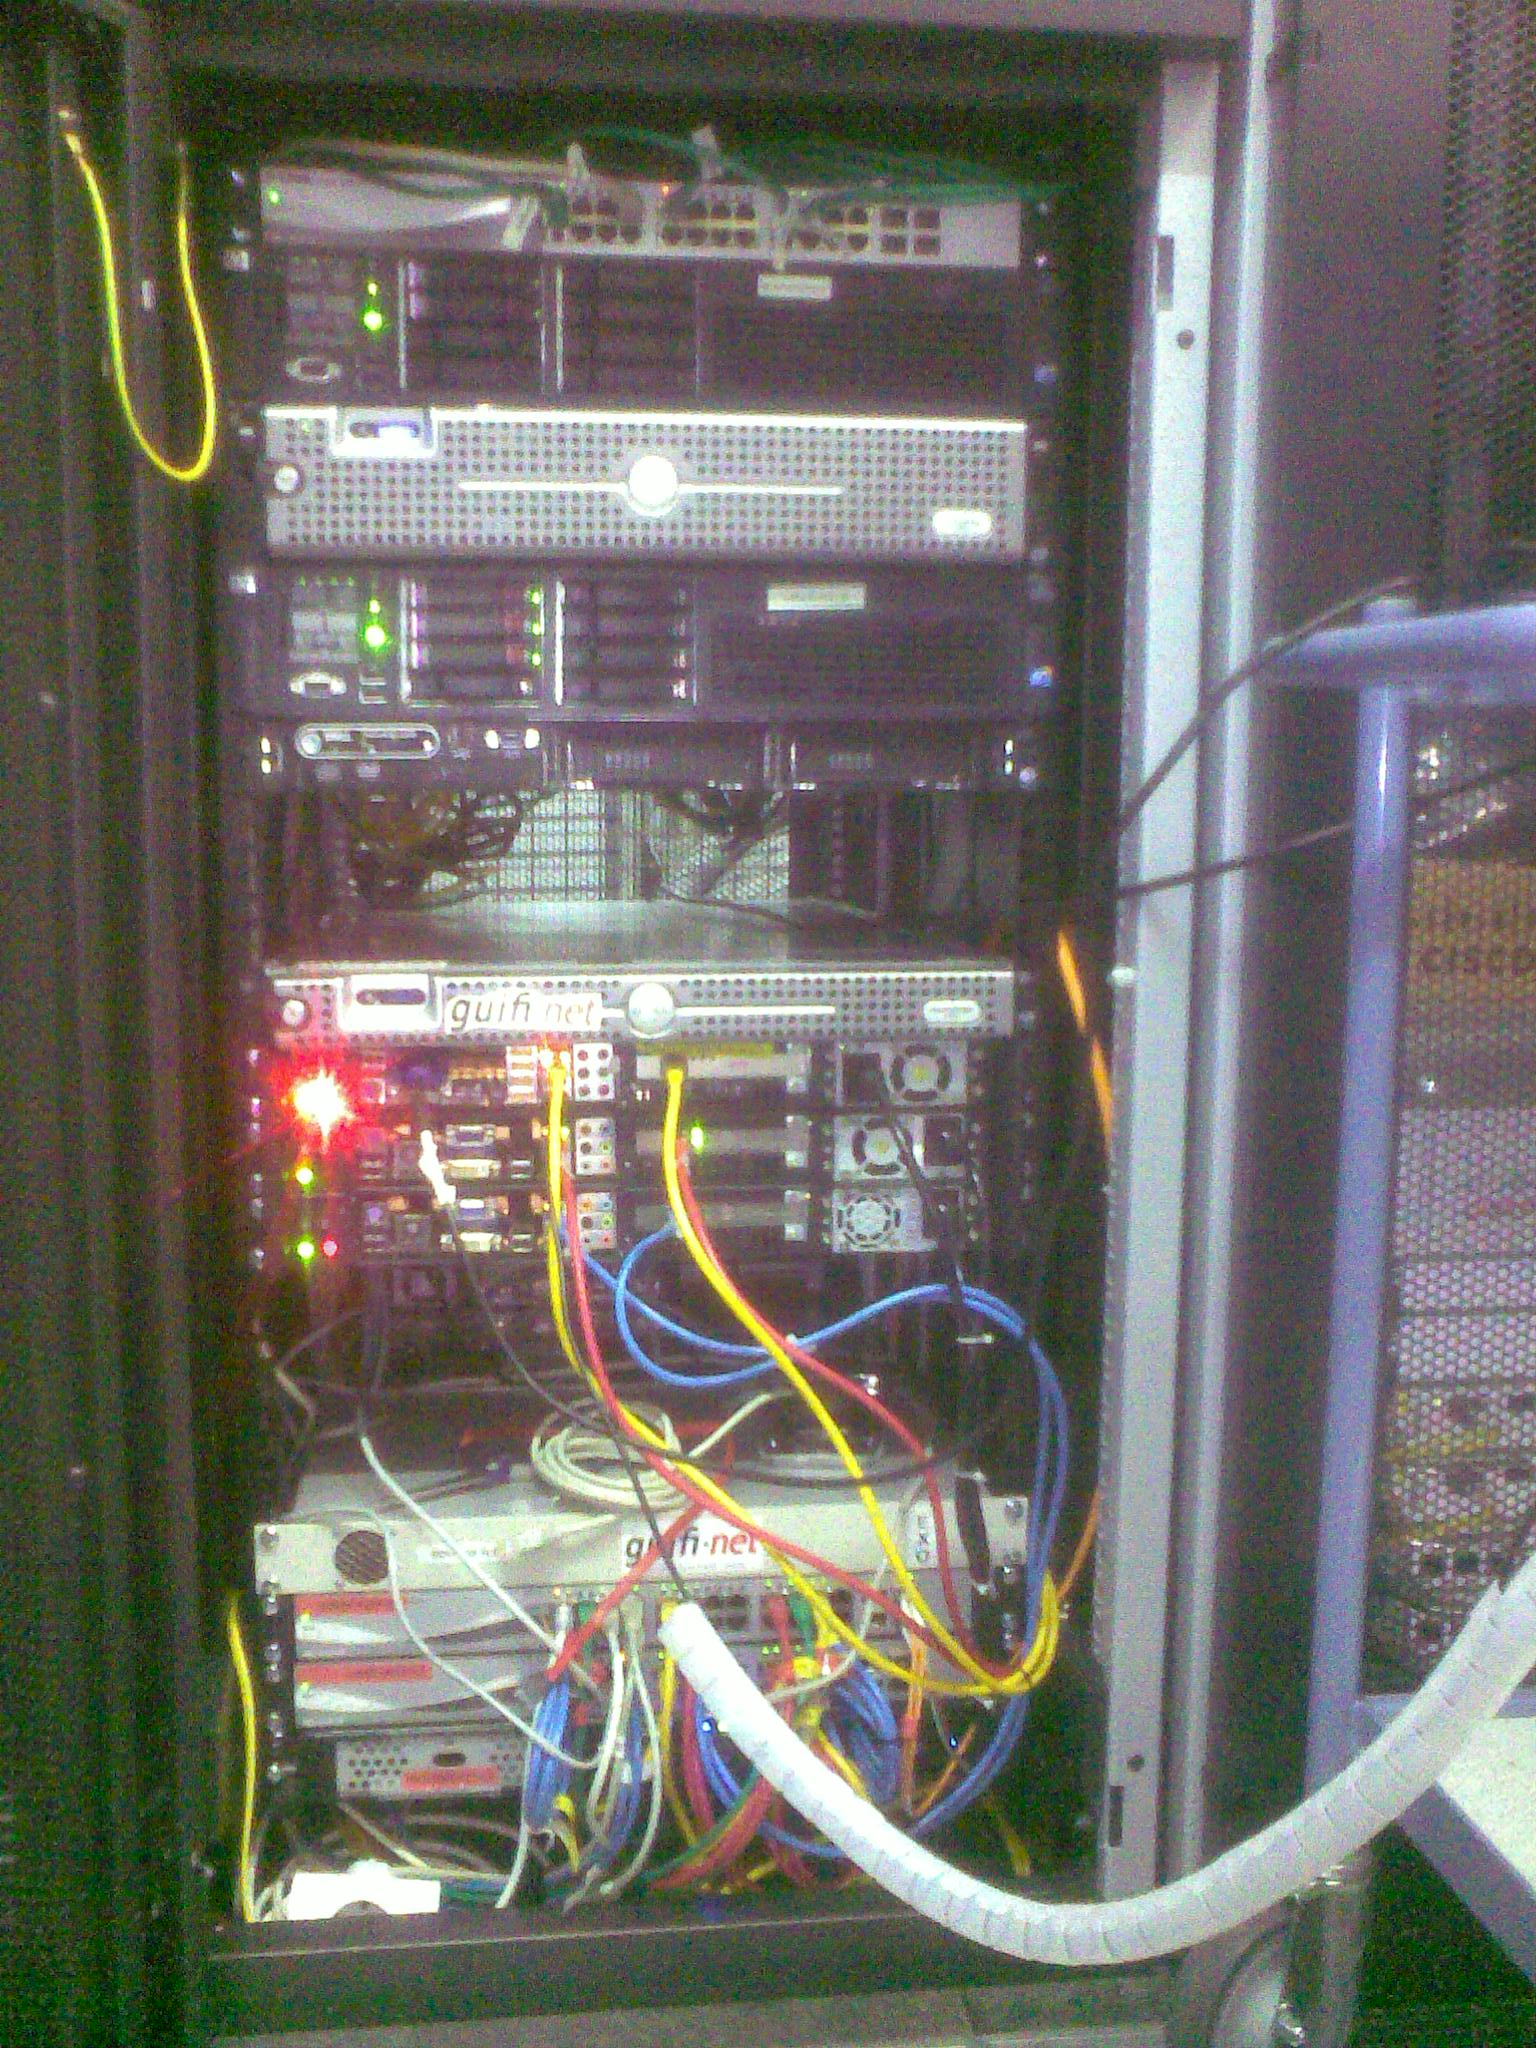
\includegraphics[scale=.65]{sect3/figures/telvent_rack_front_view.eps} 
  \caption{guifi.net Foundation rack in TELVENT-Barcelona.}
  \label{fig:telvent_rack}
\end{figure}


\begin{figure}[htbp]
  \centering
  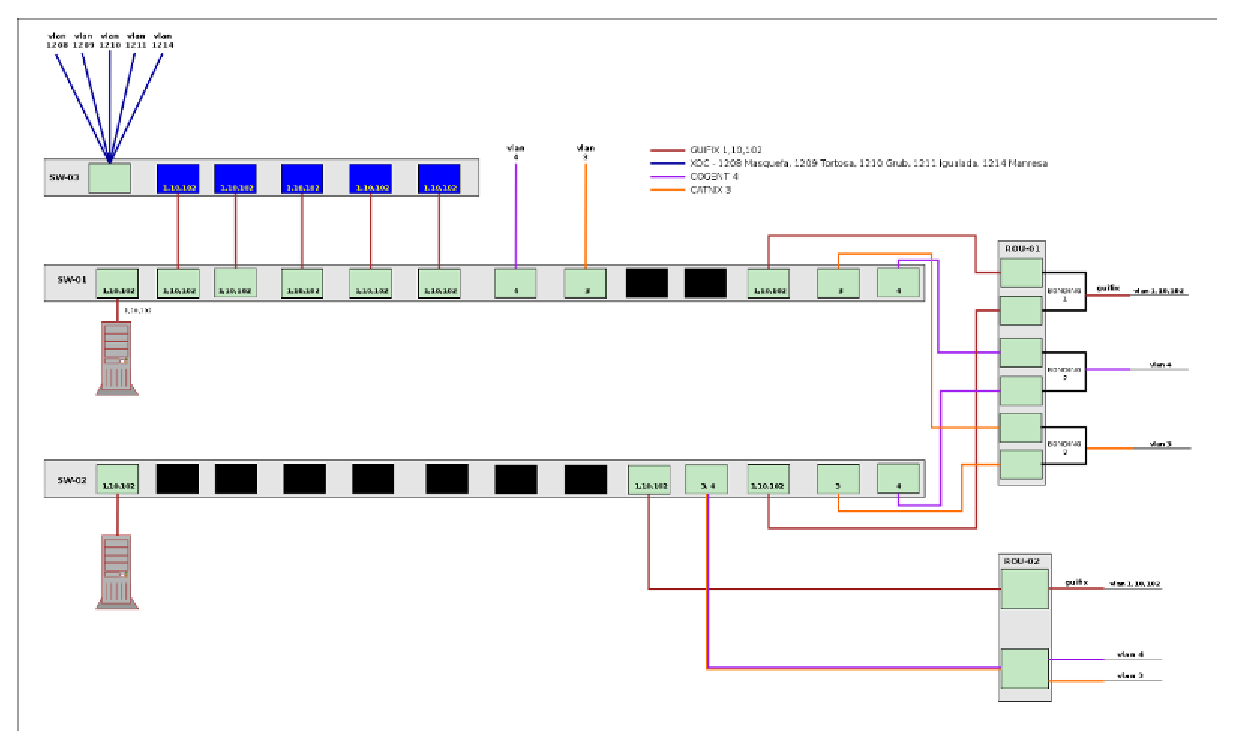
\includegraphics[scale=.75]{sect3/figures/telvent_scheme.eps} 
  \caption{CATNIX connections scheme}
  \label{fig:telvent_scheme}
\end{figure}



\FloatBarrier
\subsubsection{Masquefa}

Masquefa is a town of a rural area with a pretty high population density. Due to the poor quality of the Internet access of the traditional telcos the local government undertook a project to bring the broadband to the homes. The project was carried out and is maintained by a local SME. It combines WiFi and OF technologies and integrates a POP which was activated in 2012.

\FloatBarrier
\subsubsection{Igualda}

Igualda is a city similar to Vic. It was one of the pioneers adopting guifi.net outside Osona. The same SME which is operating the Masquefa infrastructure managed to rise a POP in this city also in 2012.


\FloatBarrier
\subsubsection{Tortosa}
Tortosa \footnote{Tortosa, population 34.432 hab, density 157,62 hab/km$^{2}$, the capital of the ''comarca'' of Anoia, Catalonia.} is a city placed on the south of Catalonia. It has a urban center similar to Vic and Igualda but additionaly has a pretty big rural area. The guifi.net users started a project named  OpenFPnet\footnote{\url{http://openfpnet.guifi.net}} with the objective of create an open and neutral fiber backbone around the surrounding villages and set up a POP, which was rised in 2012. From October 2011 to September 2012 the project was partially-funded by the Spanish government through a secondary school\footnote{Institut Montsià, \url{http://www.iesmontsia.org/}}. Currently it is economically sustained by community users grouped in associations and some local SMEs.



\FloatBarrier
\subsubsection{Expected POPs in 2013}

In 2013 other POPs are expected to be risen. The POPs that have a very high probability to happen are:

\begin{itemize}
  \item Balany\`{a}
  \item Centelles
\end{itemize} 

The POPs that can be consolidated during the 2013 are:

\begin{itemize}
  \item Aldea
  \item Matar\'{o}
  \item Cerdanyola
\end{itemize} 
